\section{Arbeitskultur}
	\subsection{Einleitung}
Bevor die Wichtigkeit der Arbeitskultur für die Beratungsdienstleistung erläutert wird, wird an dieser Stelle auf die Definition der Arbeitskultur eingegangen. Reinhard Kößler definiert den Begriff der Arbeitskultur im ``Lexikon zur Sozialogie`` von Wernern Fuchs-Heinritz als Verschiedenheit von Visionen des Arbeitsverhaltens in Form von Lebensformen, Einstellungen und Reaktionen auf die Anforderungen der Arbeit in industriell-kapitalistischen Gesellschaft. \cite{Fuchs-HeinritzLautmannRammstedtWienold1994}.
Arbeitskultur ist in der ersten Linie eine Teilmenge der Kultur (Sitten, Bräuche, Mentalität usw.) einer Nation. Gemäß Carsten Weigelt bedeutet die Arbeitskultur für die jungere Generation - sogenannten ``Digital Natives`` viel mehr als Geld und Karriere. Unter Arbeitskultur wird von ihnen das Wohl im Privatleben und am Arbeitsplatz verstanden.
Viel wichtiger ist an dieser Stelle anstatt dem Begriff von Fuchs-Heinritz die letzte Definition der Arbeitskultur von ``Digital Natives``zu betrachten. Denn für den Beratungsprozess ist es viel sinnvoller die gewünschte und die gute Arbeitskultur zu betrachten. Um festzustellen was eine gute Arbeitskultur für die IT-Beratung im internationalem Kontext ist, wurden einige Teilaspekte der Arbeitskultur definiert und abschließend werden diese Teilaspekte anhand von ausgewählten Ländern verglichen. Was beeinflusst die gute Arbeitskultur (welche Faktoren führen zum Wohl im Privat-und Berufsleben),ist es überhaupt wichtig die fremde Arbeitskultur zu analysieren, wenn man international agiert und wieweit die Beratungsdienstleistung von Arbeitskultur abhängig ist? Diese und weitere Fragen rund um IT-Beratung, sowie Arbeitskultur im internationalem Kontext werden in den nächsten Abschnitten geklärt. Es werden auch einige Probleme rund um die Arbeitskultur, IT-Beratung und den internationalen Aspekt der Arbeitskultur erläutert.\\
Die Arbeitskultur gehört zum Beratungsprozess und spielt dabei nicht die unwesentlichste Rolle. Welche Arbeitskultur gehört zum Beruf des IT-Beraters? Ein IT-Berater ist immer in der Bewegung und sein Arbeitsplatz ist nicht nur im Büro sondern auch im Zug, im Restaurant oder im Auto. Es ist sehr ersichtlich, dass die Arbeitskultur des Beraters mit der Arbeitskultur von Kunden des Beraters unzertrennlich ist. IT-Consultans kennen innerhalb der wenigsten Zeit sehr viele Firmen und deren Mitarbeiter lernen. An dieser Stelle stoßen die IT-Berater auf unterschiedlichsten Arbeitskulturen auf. Berater arbeiten oft durch Kommunikation mit Menschen aus unterschiedlichen Unternehmensebenen (Mitarbeiter, Manager, Geschäftsführer usw.), verschiedenen Branchen (Finanzdienstleistung, Fahrzeugbau, Großhandel, Chemieindustrie usw.) oder unterschiedlichen Länder mit jeweils einzigartigen Kulturen sowie Arbeitskulturen.\\
Im Vergleich zu einem Mechatroniker, der nur eine Arbeitskultur ``kennt``, konfrontieren die IT-Berater mit unterschiedlichsten Arbeitskulturen (manchmal auch international).\\
Um die Bedeutung der Arbeitskultur im internationalem Kontext für den Beratungsprozess näher zu erläutern, werden an dieser Stelle 2 Beispielfälle erklärt.\\
	 \\
	 a) Das 1. Fall ist ein IT-Consulting-Unternehmen mit eingestellten Beratern, die aus unterschiedlichen Ländern kommen, unterschiedliche Sprache sprechen und sich kulturell enorm unterscheiden. Wichtig für die Arbeitskultur an dieser Stelle ist kulturellen Gleichgewicht herzustellen und dauerhaft zu behalten. Diese Berater arbeiten zielgerichtet und ständig im Team. Im 1. Fall wird dem Autor dieser Arbeit sehr interessant, inwieweit sich kulturellen Unterschiede auf das gemeinsame Ziel des Beratungsprozesses bei der Softwareeinführung auswirken können. Auch interessant ist hier wie die IT-Berater aus unterschiedlichen Länder mit Kunden aus Deutschland umgehen, ob die kulturelle Unterschiede einen Einfluss auf Kundenbeziehungen haben oder nicht. \\
	 \\
	 b) Das 2. Fall bezieht sich auf ein deutsches Unternehmen, das sich international agiert und Kunden aus unterschiedlichen Länder betreut. In diesem Fall müssen sich deutsche Mitarbeiter auf unterschiedliche Arbeitskulturen anpassen. Denn ein Meeting während des Mittagsessen in Japan ist widersinnig und wirkt unseriös (in Japan hat das Essen einen unverletzlichen Status), in USA dagegen ist es nicht ungewöhnlich, dass beim Essen wichtige Entscheidungen kollaborativ getroffen werden.\\
	Wegen der zeitlichen sowie thematischen Begrenzung liegt der Autor dieser Arbeit den Fokus nicht auf die Differenzierung dieser zwei Fälle sowie kulturelle Unterschiede der Berater, sondern nur auf die unterschiedliche Arbeitskulturaspekte, die für den Beratungsprozess ausschlaggebend sind. Teilaspekte der Arbeitskultur, die den Autoren dieser Arbeit interessant erscheinen, werden in folgenden Kapiteln vorgestellt und verglichen. In diesem Sinne werden diese zwei Fälle nicht unterschiedlich und nur im Hintergrund behandelt.
	Diese sind aber wichtig, um zu zeigen warum die IT-Berater-Arbeitskultur nicht nur auf die deutsche Arbeitskultur sich bezieht, sondern auch im Beratungskontext einen internationalen Charakter hat.\\
	\\
\textbf{Allgemeine Arbeitsabläufe des IT-Consultings}\\ \\
	Nachdem die Arbeitskultur erklärt wurde, werden in diesem Kapitel allgemeine Abläufe des IT-Consultings detaillierter betrachtet. An dieser Stelle ist es unveräußerlich den Beratungsprozess exemplarisch zu zeigen, um die Feinheiten des Prozesses zu verstehen, die von der Arbeitskultur beeinflusst werden, um im Endeffekt Einschlüsse auf die Faktoren der Arbeitskultur zu bilden.\\ 
	IT-Consulting ist eine wichtige Art des Consultings in IT-Fragen eines Unternehmens. Das Wesen des IT-Consultings besteht im Allgemeinen darin, Unternehmen bei der Neustrukturierung der Anwendungslandschaften oder bei der Pflege der bestehenden Informationssysteme zu unterstützen. Während des gesamten Beratungsprozesses bleibt Berater als externe Experte solange im Unternehmen bis die Probleme, die er mit seinem technischen Fachwissen zu lösen hat, nicht mehr existieren oder selbständig von den Mitarbeitern des Unternehmens gelöst werden können.\\
	Um den Beratungsprozess zu verdeutlichen wird jetzt ein Beispielprozess aus der Praxis der IT-Beratung beschrieben. Ein Online-Handelsunternehmen möchte ein BI-Standardsoftware einführen und die Daten für Analysezwecke aus dem bestehenden ERP-System zu laden, um die potentiellen Kündiger zu vermeiden oder neue Kunden zu gewinnen. Am Anfang jedes Prozesses muss dem Berater die Organisationsstruktur und die Geschäftsprozessabläufe des Unternehmens klar sein, um eine passende Lösung zu finden. IT-Berater haben eine Standardsoftware im Einsatz, um geschäftlichen Probleme eines Unternehmens mit Hilfe von Informationstechnologie zu lösen. Es gibt aber keine Standardlösung die für alle Unternehmensstrukturen passend ist, weil die Unternehmensstrukturen meistens heterogen sind. Nach dem erfolgreichen Vertragsabschluss zwischen Unternehmen und der Consultingfirma beginnt die Analysephase des Beratungsprozesses. Hier wird die Unternehmensstruktur des Online-Handelsunternehmen analysiert, bis man erkennt wo die Software eingesetzt werden kann, Stellen wo die Reibungen entstehen können, welche Ressourcen stehen zur Verfügung und welches Informationssystem sich am besten für den Unternehmenszweck eignen kann. Es muss ständig ein Feedback zwischen dem Berater und Unternehmensführer oder dem Projektleiter durchführbar sein.\\
	Jetzt wird der Ablauf des Beratungsprozesses intensiver beschrieben. Nach der Analysephase beginnt man der Konzepterstellung indem für die Ideen und Pläne ein geeignetes Konzept erstellt wird. In der Folge beginnt die Umsetzungsphase, dadurch eine neue IT-Architektur aufgebaut oder die vorhandene ergänzt wird. Im unseren Beispiel wird die ERP-Lösung mit der BI-Lösung erweitert, die vorhandene Architektur bleibt erhalten. In dieser Phase können auch die andere Berater aufgerufen werden, falls es viele komplizierte Realisierungsmaßnahmen gibt.
	Nachdem das Informationssystem erfolgreich in die Unternehmensstruktur integriert ist, beginnen die Schulungsmaßnahmen, damit die Mitarbeiter des Unternehmens in der Lage sind mit diesem System umgehen zu können. Zum Schluss erfolgt die Wartungsphase und Intensität der Beratungsdienstleistung nimmt langsam ab. Diese Prozesskette kann in Form eines Lebenszyklus stattfinden.\\
	Diesen Ablauf kann man graphisch am folgenden Modell des ganzheitlichen Beratungsprozesses erkennen(seih Abb. 4.3). Dieses Modell liefert uns die einzelnen Phasen der Beratungsdienstleistung eines Freelancers im Gebiet der Managementberatung \cite{MngmBerPhasen}.


\begin{figure}[htp]
\centering
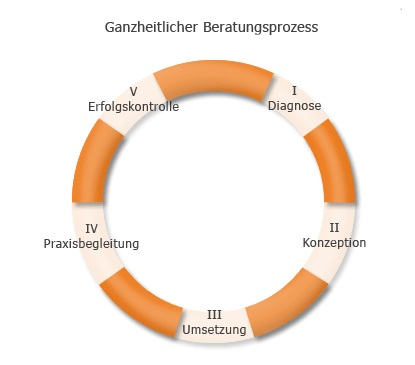
\includegraphics[width=0.7\linewidth]{./images/beratungsproz}
\caption{Phasen des Beratungsprozesses  eines Managementberaters, \cite{PhasenBeratungsprozess} }
\label{fig:beratungsproz}
\end{figure}
	
	\textbf{ Bedeutung der Arbeitskultur für IT-Consulting}\\ \\

	In wie weit ist es wichtig die Arbeitskultur für den Beratungsprozess zu betrachten? Anhand vom unseren Beispiel ist es zu erkennen, dass die IT-Berater in jeder Phase der Softwareeinführung mit den Unternehmensvertretern kommunizieren sollen. Es ist wichtig, dass die Berater genug technisches Know-how mitbringen, noch wichtiger sind die Soft Skills, die für erfolgreiche Geschäftsbeziehungen entscheidend sind. ``IT Business is People's Business``. Damit wird gemeint, dass der Erfolg von   IT-Projekten sowohl auch von den vertrauensvollen Verhandlungen maßgeblich von der Kompetenz des Beraters abhängt. \cite{ITConsRu}
	Welche Social Skills des IT-Beraters sind für Deutsche als obligatorisch nötig? Sind diese persönlichen Eigenschaften auch für die anderen Nationen von der Bedeutung? Unternehmensführung und IT-Berater müssen bei der Lösung des Problems einig werden. Der Berater muss ein Unternehmen für seine vorgeschlagene Lösung überzeugen. Muss man, um das Unternehmen zu überzeugen, nur eine gute Software anbieten und als vertrauenswürdiges Unternehmen am Markt agieren oder reichen diese Bedingungen beispielsweise in Indien nicht aus, weil der Berater möglicherweise aus anderer Kaste ist. Denn die Kastenzugehörigkeit hat in Indien bis heute kulturelle und soziale Auswirkungen auf viele Lebensbereiche \cite{KastensystemInd}.

	Für diese Arbeit ist wichtig zu wissen wie die Arbeitskultur in ausgewählten Länder sich unterscheidet und in wie weit diese den Beratungsprozess beeinflussen kann.
	In den folgenden Kapiteln wird Arbeitskultur von ausgewählten Länder(Russland,Japan, USA, Deutschland) untersucht und zum Schluss werden einige interessanten Fakten verglichen und diskutiert. 
\subsection{Teilaspekte}
	In diesem Kapitel werden die Teilaspekte von ausgewählten Ländern vorgestellt. Einige Teilaspekte werden detaillierter beschrieben, um die Wichtigkeit dieser Aspekte für das IT-Consulting hervorzuheben. Für die bessere Übersicht, um die die Teilaspekte in ausgewählten Ländern zu vergleichen, wird eine Matrix aufgestellt. Die Felder dieser Matrix bleiben zuerst leer und nach dem die einzelne Aspekte von den Ländern recherchiert und vorgestellt werden, wird die Matrix noch mal mit den ausgearbeiteten Feldern ausgefüllt, damit man daraus einen Vergleich ableiten kann. Die Recherche findet in 3 Sprachen (Deutsch, Englisch und Russisch) statt, um den Fokus der Recherche zu verbreiten.
	
\begin{table}[htp]
\begin{tabular}{|c|c|c|c|c|c|}
\hline  Aspekt/Land& Deutschland & USA & Russland & Japan & Indien \\ 
\hline 	Hierarchien  & ? & ? & ? & ? & ? \\ 
\hline  Gehalt& ? & ? & ? & ? & ? \\ 
\hline  Gesetze& ? & ? & ? & ? & ?  \\ 
%\hline  Grad des intuitiven Handelns& ? & ? & ? & ? & ? & ? \\ 
\hline  Kritikfähigkeit& ? & ? & ? & ? & ? \\ 
\hline  Team& ? & ? & ? & ? & ?\\ 
\hline  Entscheidungsfindung& ? & ? & ? & ? & ?  \\ 
\hline  Lebensstandard& ? & ? & ? & ? & ? \\ 
\hline  Pünktlichkeit& ? & ? & ? & ? & ?\\ 
\hline  Arbeitszeit, Urlaub, W-L-B& ? & ? & ? & ? & ?\\ 
\hline 
\end{tabular} 
\caption{Matrix der Arbeitskultur}
\end{table}
%Ende der Recherche-> Information für neue Matrix
%1)Hierarchien und Organisation->Hierarchien 2)Kundenverh weg 3)spezielle Rechtslage->Gesetze 4)Grad des intuitiven Handelns weg 5) Kritikfähigkeit nur bei Japan,De 6) Lebensumstände ->Lebensstandards ->Zeitmanagement in Form von Pünktlichkeit 7)Work-Life-Balance-> Arbzeit und Urlaub 8)Entsch.findung nur Russland
%
%Durch einer Recherchewerden einige Teilaspekte verändert. Dafür gibt es mehrere Gründe, bspw. waren die recherchierten Teilaspekte besser formuliert oder einige waren in ihrer Definition zu weit gefasst und müssten demzufolge zusammengefasst werden. Für bestimmte Teilaspekte gibt es keine Information, die durch Recherche in 3 verschiedenen Sprachen (Deutsch, Englisch und Russisch) nicht zu finden ist. An dieser Stelle besteht noch Forschungsbedarf. 
Dieses Kapitel hat im Vergleich zu den Kapiteln ``Markt`` und ``Bildung`` eine andere Struktur, indem nicht nach den Teilaspekten der Arbeitskultur gegliedert wird. Dafür wird hier eine Unterteilung des Kapitels nach Ländern vorgenommen und in diesen werden die Teilaspekte wie Hierarchien, Gesetze oder Team beschrieben.
Bevor die ausgewählten Ländern untersucht werden, definiert man in folgenden Kapiteln zuerst die wichtigsten Teilaspekte der Arbeitskultur.

\subsubsection{Gehalt}
Gehalt ist einer der wichtigsten Faktoren für die angenehme Arbeitskultur. Diejenigen, die ein gutes und faires Gehalt bekommen sind motiviert, meist zufrieden mit ihrem Job und aus psychologischer Sicht sind sie sicher, dass sie für eigene Mühe ein gerechtes Gehalt bekommen. Demzufolge hat das Geld nicht nur die Tauschmittel-Funktion (es erlaubt uns,das zu kaufen, was wir zum Leben brauchen), sondern auch eine psychologische. Laut Täubner steht das Geld für Erfolg, Sicherheit, Anerkennung, Macht, Lebensqualität und Selbständigkeit \cite{GehaltBedeutungDE}.\\
Wenn die Arbeitnehmer im Gegensatz zum guten Verdienst mit ihrem Gehalt unzufrieden sind, dann gibt es meist kein Wohl am Arbeitsplatz. Es lässt sich doch sagen, dass das Geld nicht der wichtigste Faktor für gute Arbeitskultur ist. Laut der StepStone-Studie,in der rund 18.500 Fach- und Führungskräfte befragt wurden, um zu wissen was die Arbeitnehmer am meisten motiviert, steht das Geld nur auf dem 3.Platz nach dem guten kollegialen Arbeitsumfeld und dem Spaß am Arbeiten \cite{GehaltNR.3DE}.\\
 Schlussendlich lässt sich sagen,dass das Gehalt ein wichtiger Motivierungsfaktor ist, der allein zu schwach ist, um eine gute Arbeitskultur zu gewährleisten.
IT-Berater sind daher keine Ausnahme, wenn es um Gehalt geht. Berater arbeiten viel und meisten möchten dafür gut verdienen. Die Arbeitszeiten von IT-Berater werden im nächsten Kapitel vorgestellt.\\
Interessant zu wissen ist noch, wie sich das Gehalt von IT-Beratern in den ausgewählten Ländern sich unterscheidet und in wieweit er deren Arbeitskultur beeinflusst.
\subsubsection{Arbeitszeit, Urlaub, Work-Life-Balance}
Flexible Arbeitszeiten und viele Urlaubstage sind wichtigsten Faktoren um die Work-Life-Balance zu bestimmen. Dazu zählen noch laut Feddersen: die Möglichkeit im Homeoffice zu arbeiten, Zeit für Fortbildung und Kinderbetreuung \cite{WLB}.\\
Work-Life-Balance ist heute kein leerer Begriff mehr. Das, was dahinter steht, gewinnt zunehmend an der Bedeutung. Arbeitnehmern sowie Arbeitgebern wird immer bewusster, dass die Work-Life-Balance nicht nur die Balance zwischen Job und Privatleben ist, sondern auch ein wichtiger wirtschaftlicher Faktor. Die Work-Life-Balance beeinflusst die Arbeitskultur und auch die Arbeitsleistung sowie die Produktivität von Mitarbeitern, was für Arbeitgeber entscheidend ist, um das Gleichgewicht zwischen Berufs- und Privatleben für Angestellten zu gewähren. Die Vorbeugung von Burnout-Erkrankungen ist dabei sicherlich ein weiterer, positiver Nebeneffekt. \cite{WLB} \\
Das Gleichgewicht zwischen Berufs- und Privatleben herzustellen, ist für IT-Berater nicht einfach. Denn IT-Berater sind ständig auf Reißen, arbeiten 60-70 Stunden pro Woche und diese Arbeit ist meist sehr geistig anstrengend \cite{WLBbeiIT-Berater}. Für junge IT-Berater könnte es kein Problem sein, wie sieht es aus wenn man eine Familie und Kinder hat? Laut Robert Laube, der für Service Line ``Business Intelligence`` bei Avanade verantwortlich ist, erfordert die Work-Life-Balance sehr viel Selbstdisziplin \cite{WLBbeiIT-Berater}. Dazu gehört beispielsweise die Verbannung von E-Mails auf dem Handy oder ``[...] morgens mit den Kindern zu frühstücken und sie in die Schule und den Kindergarten zu bringen`` falls es die Zeit erlaubt \cite{WLBbeiIT-Berater}.

\subsubsection{Lebensstandard}
Der Lebensstandard in den ausgewählten Ländern gehört auch zum wichtigen Teilaspekt der Arbeitskultur. Es ist vor allem wichtig das Gehalt von IT-Berater im Bezug zum Lebensstandard in einem bestimmten Land zu betrachten. Mit anderen Wörtern kann man den Lebensstandard als Ergänzung zum Gehalt oder als Ergänzung zu der Währung sehen, um das Gehalt in den ausgewählten Ländern objektiver zu vergleichen. An dieser Stelle ist es sinnvoll ein Beispiel zu erwähnen, um den Sachverhalt zu verdeutlichen. IT-Berater aus Deutschland verdienen durchschnittlich mehr als ihre russischen Kollegen, doch sind die Lebenshaltungskosten wie Nahrung, Miete, Kleidung in Russland geringer als in Deutschland.\\
Im Allgemeinen beschreibt der Lebensstandard den sozio-kulturellen Wohlstand von Personen im Verhältnis zu Vergleichspersonen innerhalb einer kulturellen Gemeinschaft. Bestimmt wird dazu die jeweilige Höhe der Lebensbedingungen bzw. die Befriedigung von materiellen und geistig-kulturellen Bedürfnissen. \cite{LbsWiki} \\
Natürlich unterscheiden sich die Faktoren, die den Lebensstandard in ausgewählten Ländern beeinflussen. Es ist aber wichtiger für dieser Arbeit zu wissen, dass der Lebensstandard den Gehalt von IT-Beratern beeinflusst und damit die Arbeitskultur von Beratern , und nicht den internationalen Unterschied von einzelnen Lebensstandardindikatoren.

%\subsubsection{Team}
\subsection{Analyse der ausgewählten Teilaspekte}

	\subsubsection{Russland}

	
	\textbf{Einleitung}\\ \\
	Der Aspekt-Markt spielt für die Arbeitskultur nicht die unwesentlichste Rolle. Zwischen diesen Aspekte gibt es einige Zusammenhänge wie das Gehalt oder die Arbeitszeiten von IT-Berater.\\
	Russland ist ein Wachstumsmarkt mit Zukunft. Laut Holger Hirsch ist heute der damals geschützter russischer Markt offen für Exporte und Investitionen aus Deutschland. Dies gilt sowohl für IT-Beratungs-Unternehmen, die ihre Softwareprodukte in Russland integrieren auch für russische Manager, die bei der Informationstechnologie auf westliches Know-how setzen.\cite{ITConsRu}\\
	Da der Markt für IT-Beratung neu ist, muss man als IT-Berater aus Westen ganz viele Entscheidungen intuitiv treffen. Hier weden natürlich die Soft Skills des Beraters gefragt. Technische Fähigkeiten, funktionales Wissen und Branchen-Know-how sind selbstverständlich vorausgesetzt. Sonst wären die höheren Gehaltstarife für westlichen Berater ungerechtfertigt. Mit anderen Wörtern müssen deutsche Beratern ein breiteres Wissen besitzen als ihre russischen Kollegen, um möglicherweise an den russischen Softwareprojekten teilnehmen zu können. ´´Der Zerfall der Sowjetunion und die Reformen im wirtschaftlichen und sozialen Gefüge Russlands haben einen erheblichen Einfluss auf die Arbeitskultur in gegenwärtigen russischen Organisationen´´\cite{ProzessbeglBerRU}.
	Deswegen überlappen sich die kulturelle mit reformbedingten Faktoren der Arbeitskultur. Es ist daher sehr schwer den Ursprung dieser Faktoren zu unterscheiden. Am Beispiel des russischen Kollektivs könnte diese Überlappungen der russischen Kultur und sowjetischen Reformen ersichtlich werden. Autor dieser Arbeit möchte an dieser Stelle auf Beschreibung von Teilaspekten der Arbeitskultur eingehen und nicht auf die detaillierten Erklärungen von den Ursachen der Entstehung der Teilaspekte, solange es nicht im Kontext des IT-Consultings relevant ist.\\ \\

	\textbf{Gehalt}\\ 
	\\
	Der russischer Senior-Consultant aus Moskau verdient im Mittel 3845 € monatlich. Das ist für russische Verhältnisse relativ hoher Gehalt. Zum Vergleich beträgt der durchschnittlicher Gehalt in Russland beim aktuellen Währungskurs 587,60 €(in Moskau 927.57 €) \cite{RusGehAllgm}. Es gibt  in Russland sehr starke regionale Gehaltsunterschiede. Aus dem unten stehenden Diagramm kann man den Unterschied des monatlichen Gehalts für SAP-Berater ermitteln. Im Großen und Ganzen verdient man in beiden Metropolen Moskau und Sankt-Petersburg ca. das doppelte wie in anderen Großstädten wie Rostov, Wolgograd oder Omsk.
	\\
\begin{figure}[htp]
\centering
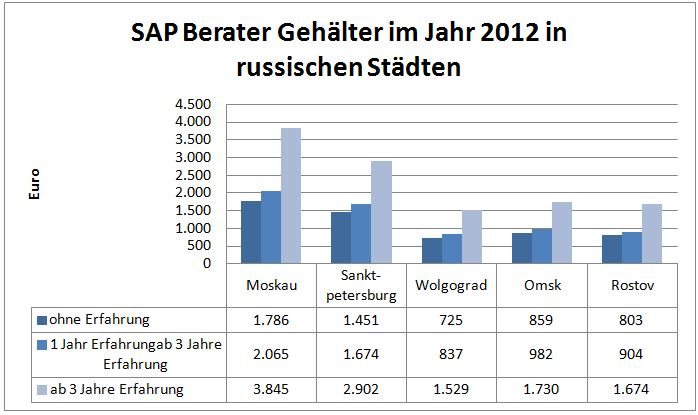
\includegraphics[width=0.7\linewidth]{./images/SAP-Berater_Gehalt_RU}
\caption{SAP-Berater Gehälter in Russland \cite{GehaltSAPBerRU}}
\label{fig:SAP-Berater_Gehalt_RU}
\end{figure}
\\
%Quelle:http://www.tadviser.ru/index.php/%D0%A1%D1%82%D0%B0%D1%82%D1%8C%D1%8F:%D0%A0%D1%8B%D0%BD%D0%BE%D0%BA_%D1%82%D1%80%D1%83%D0%B4%D0%B0_%D0%B2_%D0%A0%D0%BE%D1%81%D1%81%D0%B8%D0%B8_(%D0%98%D0%A2_%D0%B8_%D1%82%D0%B5%D0%BB%D0%B5%D0%BA%D0%BE%D0%BC)
	Senior IT-Berater aus Deutschland verdient zum Vergleich durchschnittlich 6.250 € im Monat\cite{GehaltSAPBerDE}. Der Junior Berater im IT Umfeld ohne Projekterfahrung  verdient in Russland durchschnittlich 1200 € monatlich\cite{GehaltSAPBerRU}. Laut der russischen Arbeitsagentur ``rabota.ru`` steigt die Anfrage auf ERP-Systemen enorm und deswegen steigen auch die Gehälter für Spezialisten in diesem Umfeld. Die Anfänger im IT-Beratungsbereich sind bereit am Anfang der Karriere fast kostenlos zu arbeiten, um Gold werte  Erfahrungen im ERP-Bereich zu sammeln \cite{RusGehRabota}.
	Der deutsche Junior-Berater mit den gleichen Qualifikation und Erfahrung verdient ca. drei mal so viel (3750 €) \cite{GehaltSAPBerDE} als sein russischer Kollege.\\ \\
	\textbf{Team: %und Organisation: 
	Russischer Arbeitskollektiv gegen westlichen Team}\\
	\\
	``Das Arbeitskollektiv wurde in der sowjetischen 
	Epoche als das zentrale soziale Handlungsfeld propagiert. Es repräsentiert,dass die Geschlossenheit der Gruppe wichtiger als die Selbstverwirklichung der einzelnen Gruppenmitglieder`` ist.\cite{ProzessbeglBerRU}\\
	Gruppeninterne Konflikte wurden deshalb weniger vermieden oder nicht diskutiert. Der Unterschied gegen dem westlichen Team besteht darin, dass russischer Kollektiv eine dauerhafte Einrichtung mit klar zugewiesenen Leitungskompetenzen ist, die vom Vorgesetzten häufig ausgeübt werden. Im Gegensatz zum russischen Kollektiv wird das westliche Team nur für die Dauer eines bestimmten Projektes eingerichtet und zeichnet sich durch die Gleichberechtigung aller Teammitglieder aus.\\
	So ein Kollektiv für Beratungszwecke ist demzufolge oft nicht flexibel und ist zu stark weisungsgebunden. Die Aufgaben im Kollektiv werden meistens vom Vorgesetzten vorgeschrieben, im unser Fall von einem Projektleiter oder einem Manager. Solche Führungspersonen sind im IT-Beratungsfall oft an dem Büro gebunden und sind meistens in diesem Büro während die Berater oft unterwegs bei den Kunden sind. Daher müssen die Entscheidungen intuitiv und unabhängig von dem Vorgesetzten getroffen werden. Die Tatsache, die Entscheidungen intuitiv zu treffen, spiegelt sich dem Prinzip des russischen Kollektivs wieder.  ``Russische Organisationen zeichnen sich durch eine Konzentration von Macht auf die Führungskräfte aus. Ohne den Vorgesetzten werden keine Entscheidungen getroffen``. \cite{ProzessbeglBerRU} \\
	Verlagerung von Entscheidungen auf die Mitarbeiter wird in Russland selten stattfinden, deswegen werden die Mitarbeiter von den Führungskompetenzen befreit und übernehmen oft nur Ausführungsanweisungen. Für  den Beratungsprozess ist diese Tatsache ein reisen Minuspunkt, weil die Berater das interdisziplinäres Wissen besitzen und  den vollen Handlungsspielraum in der IT-Beratungsszene brauchen.
	Zu erwähnen wäre noch, dass die jungen Menschen von solcher Stereotypen weiter entfernt sind als die ältere ``sowjetische`` Generation. \\ \\
	\textbf{Gesetze: Personalauswahl und russische Gesetze}\\
	\\
	 Eine weitere wichtige Besonderheit ist die Personalauswahl. Häufig erfolgt die Auswahl von neuen Mitarbeitern nicht nach Kriterien der fachlichen Kompetenz. Oft werden Arbeitsplätze unter Verwandten und 
	 Freunden vergeben. Es existieren fast keine etablierten Mechanismen von Angebot und Nachfrage auf dem Arbeitsmarkt. Vakanzen werden häufig nicht an den fachlich geeignetsten Bewerber vergeben, sondern an ``unseren Mann``(nash chelovek). Sinngemäße Übersetzung bedeutet, dass ``Unser Mann`` oder ```nash chelovek`` eine besondere, meist verwandtschaftliche Beziehung zum Unternehmensführer oder den Vorgesetzten des Unternehmens hat.\\
	 Ein weiteres für russische Arbeitskultur typisches Merkmal ist, dass die Gesetze, Bestimmungen und Regelungen keinen eindeutig verbindlichen Charakter haben. In Abhängigkeit von der Situation und den involvierten Personen, können Regeln oder Gesetze bewusst unberücksichtigt bleiben. Wie sich jedoch diese Abstufung darstellt ist nicht vorhersagbar. Das liegt auch daran, dass das russische Volk und die russischen Behörde sich einander nicht zutrauen. Die Strenge des Gesetzes wird oft in der Vernachlässigung der Gesetzgebung ausgeglichen. \cite{ProzessbeglBerRU}\\ \\ 
	 \textbf{Arbeitszeit, Urlaub, Work-Life-Balance}\\ %Work-life-Balance gehört dazu
	 \\
	 Die gesetzliche Wochenarbeitszeit in Russland beträgt 40 Stunden. Doch in meisten Fällen wird diese Grenze total überschritten. Die IT-Spezialisten arbeiten zwischen 10 und 11 Stunden am Tag in einem 5-Tage-Rhythmus \cite{ArbZeitRU}. 
	  Oft wird auch eine 6-Tage-Woche praktiziert. Zum Vergleich arbeiten deutsche IT-Berater oft weniger (sieh Kapitel-Deutschland ``Arbeitszeit und Urlaub``) und die wöchentliche Arbeitszeit der japanischen Kollegen(sieh Kapitel-Japan ``Arbeitszeit und Urlaub``) ist am längsten in den ausgewählten Ländern. 
	 In vielen Tarifverträgen in Deutschland beträgt der Jahresurlaub 30 Arbeitstage. In Russland sind es dagegen nur 24 Tage. Der Arbeitstag beginnt bei russischen nicht produzierenden Firmen um 9 oder 10 Uhr \cite{ArbZeitRU}. Wenn ein IT-Berater um 10 Uhr mit seiner Arbeit beginnt, dann ist er vermutlich um 20-21 Uhr zu hause. Daraus lässt sich schlussfolgern, dass es aufgrund der Zeitmangel auf die persönliche Bereiche wie die Freunde, Familie und Work-Life-Balance von russischen Beratern eine negative Auswirkung gibt.   \\ \\
	 \textbf{Pünktlichkeit und Reisen }\\
	 \\
	 Der IT-Berater-Beruf ist eine Tätigkeit, die mit höheren Reisebereitschaft verbunden ist, Beratung heißt meist, beim Kunde vor Ort zu sein. In Deutschland sind die Berater ganz oft mit Autos unterwegs. Von einem deutschen Großstadt bis zum anderen braucht man beispielsweise 4-5 Stunden. In Russland gibt es 2 grundsätzliche Transportprobleme mit dem Consulting-Hintergrund, die dem Autor auf den Ersten Blick erscheinen: Staus in Moskau und große Entfernungen zwischen den russischen Städten. Nachfolgend wird der Autor diese 2 Probleme näher erläutern. Das Land ist sehr groß und weit (es umfasst 11 Zeitzonen).
	 Zwischen Moskau und Nowosibirsk sind es ca 4 Stunden nur Flugzeit plus 3 Stunden Zeitunterschied. Wenn ein Berater aus Moskau seinen Arbeitstag am Montag in Nowosibirsk beginnen möchte, muss er schon am Sonntag ausreißen. Die Reisen sind erschöpfend und könnten von russischen Berater,die eine Familie haben, nicht so gern angenommen. Für diese Familienleute stören auch die Work-Life-Balance von IT-Beratern, weil die Reisen direkt ins Privatleben eingreifen und sehr viel wertvollen Zeit kosten.\\
	 Laut dem russischen Rating "Consulting research" aus 21 größten IT-Consulting-Unternehmen befinden sich 13 Unternehmen in Moskau\cite{RaitConsRU}.
	 Aus 100 größten russischen IT-Unternehmen befinden sich in Moskau 71 Firmen \cite{100BigITConsURU}. 
	 Moskau ist nicht nur ein teuerster Hauptstadt der Welt und ein wirtschaftliches Zentrum des Landes, sondern auch ein strategisches Standort für IT geworden.
	 Mit der Stadtwachstum werden die Staus länger und länger.``Nach Angaben des GPS-Navigationsanbieters TomTom ist Mosaku Nummer eins unter den schlimmsten Stau-Städten der Welt\cite{MoskauStau1}.``
	 Da die Berater öfters unterwegs sind, ist es eine große Anstrengung in Moskau Auto zu fahren. Um von A nach B zu kommen wird ganz oft ein Metro benutzt. 
	 Deswegen ist es in Moskau ``erlaubt`` dem Berater sowie allen Geschäftsleuten ein Viertel bis halbe Stunde zum Meeting oder zum  Kunde zu spät zu kommen. Oft werden Staus als Ausrede, die auch akzeptiert wird, genutzt.\\
	 Allgemein zählt die Pünktlichkeit nicht zu den Stärken von Russen: die Termine werden nicht immer eingehalten, E-Mails werden nicht sofort beantwortet und die Versprechungen sind nicht immer realistisch. Deswegen muss man als Berater diese Verzögerungen mit einplanen \cite{RusKnigge}.\\ \\
	 	 \textbf{Hierarchie und Entscheidungsfindung}\\
	 	 \\
	 Im Teilaspekt Organisation hat der Autor erwähnt ,dass in russischen Organisationen der Chef oder sogenannte Generaldirektor  allein das Sagen hat. So beschreibt auch der Sergey Frank, dass die Entscheidungskompetenzen in Russland nicht wie gewöhnt nach unten gehen, sondern nur der Geschäftsführer die Entscheidungsbefugnisse hat \cite{RuSFI}.
	 Deswegen kommunizieren die russische IT-Berater oft nur mit dem Geschäftsführer des Unternehmens, was natürlich zur zeitlichen Verzögerungen im Projekt führen kann.\\
	 Gemäß ``Russland-Knigge`` \cite{RusKnigge} werden oft die Hierarchien in Russland nicht eindeutig und nicht klar erkennbar. Die Berater müssen schon vor Beginn der Verhandlungen herausfinden, wer das entscheidende Wort hat. Damit wird keine Zeit durch unnötige Gespräche mit Personen, die möglicherweise keinen Einfluss auf den Verhandlungsverlauf haben, verloren.\\
	 Laut ``Businessknigge Russland`` sind ``die Flache Hierarchien nicht die Sache der Russen`` \cite{RusKnigge}. Es heißt, dass auf der Ebene in der Geschäftsstruktur unter dem Unternehmensführer  sehr viele anderen Personen sein könnte, die einerseits zum Geschäft gehören, anderseits ist die Zusammengehörigkeit dieser möglichen Personen zum Geschäft sowie deren Aufgabengebiet meistens nicht klar definiert ist. An dieser Stelle in der Unternehmensstruktur könnte oben beschriebener ``nash chelovek`` auftauchen.
	\\ \\
		 	 \textbf{Lebensstandard}\\ \\
	Laut den Ergebnisse von Umfragen, die von der russischen Agentur für Finanzforschungen (russ. Abk.: NAFI) in den Jahren 2004 bis 2011 durchgeführt wurden, hat sich die materielle Lage der russischen Bürger in den vergangenen  Jahren trotz der Krise von 2008 und 2009 allmählich verbessert.\\
	 Die sogenannte „Vormittelklasse“, zu der fast die Hälfte aller Einwohner Russlands gehört, bestätigte einen Wachstumstrend. Dabei handelt es sich um Bürger, die genug Geld für Lebensmittel und Kleidung haben, denen jedoch der Kauf von langlebigen Waren schwer fällt. Laut der Meinungsforschung betrug diese Menschengruppe vor sieben Jahren nur höchstens 30 Prozent der Bevölkerung. In den letzten 7 Jahren ist der Anteil der armen Bürger an der Landesbevölkerung von 14 \% in 2004 auf 5\% in 2011 gestiegen. Auch die Gruppe der Einwohner, denen das Geld für die Nahrungsmittel, nicht aber für die Kleidung ausreicht, ist von 35 \% in 2004 auf 28 \% in 2011 zurückgegangen.\\
	 Trotzdem lässt sich sagen, dass es immer noch enorme finanzielle Unterschiede zwischen der reichen und armen Bevölkerung in Russland gibt. Der durchschnittliche Gehalt in Russland beim aktuellen Währungskurs beträgt 587,60 € (in Moskau 927.57 €). Es ist noch zu erwähnen, dass die kleine Gehälter mit dem niedrigen Lebenshaltungskosten wie gesetzliche Ausgaben, Nahrung, Kleidung usw. ausgeglichen werden. 
	\subsubsection{Japan}
	\textbf{Pünktlichkeit, Kritik und Besonderheit der Kommunikation}\\
	\\
	Im Geschäftsleben sind die Japaner besonders pünktlich. Pünktlich bedeutet in diesem Fall 5 bis 10 Minuten vor einem Termin zu erscheinen. Selbst nur bei 5 Minuten Verspätung müssen Sie an Ihren Geschäftspartner Bescheid geben, dass Sie sich verspäten. \cite{JPKnigge}. \\
	Die Kritik wird in Japan nicht direkt, sondern ausweichend und über den ``Umweg`` geäußert. Diese Kritikäußerung-Strategie wird auch von ausländischen Geschäftspartner erwartet. Eine Besonderheit in Japan hat die Bedeutung des Wortes ``Ja``: in einem Gespräch reagiert man mit ``Ja`` nicht auf die Zustimmung mit der Sache, sondern auf die Bestätigung des Zuhörers \cite{JPKnigge}. Ein lang-gesprochenes ```Ja`` bedeutet die Zustimmung vom bestimmten Sachverhalt.\\
	\\
	\textbf{Hierarchie und Rangordnung}\\
	\\
	Im japanischen Geschäftsleben spielt die Rangordnung eine wichtige Rolle.
	Beim Essen sitzt die wichtigste Person in der Mitte der Reihe, je größer die Entfernung von ihr, desto geringer der Rang \cite{Business-KniggeFernost}.	
	Beim Meeting wird der Ranghöchster zuerst sprechen. Bei der Begrüßung wird zuerst die Hand nicht der Frau gegeben wie das in Deutschland üblich ist, sondern dem Ranghöchsten. \\
	\\
	\textbf{Arbeitszeit, Urlaub, Work-Life-Balance}\\
	\\
	Offiziell gilt in Japan 40-Stunden-Woche, in der Realität sind Angestellten bis 21 oder 23 Uhr im Büro. Wenn jemand eher nach Hause geht als sein Chef, muss bei der nächsten Beförderung mit Konsequenzen rechnen \cite{ArbZeitJP}. Den Arbeitsplatz eher als der Chef zu verlassen zählt in Japan zu den schlechten Manieren im Geschäftsleben.
	Der Überschrift eines Online-Zeitungsartikels ``Im Japan arbeitet man sich bis zum Tode`` hat sich schon lange als Stereotyp in Japans etabliert. 
	16 Stunden am Tag im Büro, Schlafkammer, Mittagsschläfchen im Zug, unzählige Überstunden gehören zum modernen Arbeitsalltag in Japan. ``Schuld daran haben die Zeitarbeitsagenturen, denn ca ein Drittel der japanischen Arbeiterschaft besteht aus Zeitarbeitern``, sagt der amerikanische Journalist Jake Adelstein \cite{JPArbeit}. Im Gegensatz zu Deutschland, wo die Überstunden nicht immer gezahlt sind, werden in Japan die Überstunden zu der zusätzlichen Geldquelle, ohne dieser man schwer überleben kann.
	Es wurde keine Quelle gefunden, um die Arbeitszeit der IT-Berater zu bestimmen. Da kann der Autor nur persönlich vorstellen, dass 4-Tage-Woche beim Kunde mit einem zusätzlichen Tag für Meetings in der Firma bei den deutschen Berater ein Paradies für japanischen Kollegen sein kann. \\
	In Deutschland genießen die Arbeitnehmer 30 Tage einen bezahlten Urlaub. In den USA beträgt Jahresurlaub rund 2 Wochen. Offiziell sind in Japan im Durchschnitt 17 Freitage gewährt, allerdings werden nur 8 Tage im Krankheitsfall in Anspruch genommen. Weil während des Urlaubs keine Lohnfortzahlung stattfindet, muss ganz oft Urlaub unter einer Krankheit ``versteckt`` werden \cite{JPArbeitSozKultur}. Denn die Abwesenheit im Krankheitsfall wird vom Unternehmen akzeptiert und Lohnfortzahlung wird geschehen.\\
	\\
		\textbf{Gesetze: Steuer und Sozialausgaben}\\
		\\
		Steuern und Sozialabgaben sind in Japan niedriger als in Deutschland. Japanischer Mehrwertsteuer beträgt im Gegensatz zu Deutschland nur 10 \%.
		``Als Arbeitnehmer ist man in Firmen mit mehr als fünf Angestellten durch eine sog. Employee Health Insurance abgesichert``. Jedoch muss man 10 bis 30 Prozent der Behandlungskosten aus eigener Tasche zahlen. Die Arbeitslosenkosten übernimmt der Arbeitgeber \cite{ArbZeitJP}. \\
	\\
			\textbf{Lebensstandard}\\
			\\
		\\Der Lebensstandard in Japan ist vergleichbar mit dem mitteleuropäischen (sieh Abb.4.4).
		\begin{figure}[ht]
		\centering
		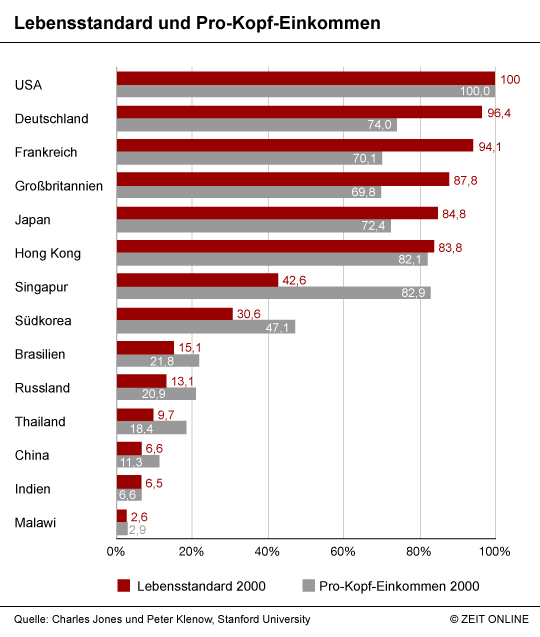
\includegraphics[width=0.7\linewidth]{./images/Lebensstandard-Pro-Kopf-Einkommen}
		\caption{Lebensstandard und Pro-Kopf-Einkommen \cite{LebensStd}}
		\label{fig:LebStdProKEink}
		\end{figure}\\
		Gemäß Miroslav Stimac sind die Ausgaben der Grundbedürfnisse in Deutschland höher als in Japan \cite[101]{Stimac2004}.
		Beispielsweise kostet Nahrung in Tokio durchschnittlich 2,36 mal mehr als in Deutschland. Viele japanische Städte leiden an Platznot, dies führt zu hohen Grundstückspreisen sowie Mietpreisen \cite[105]{Stimac2004}.
		Eine Familie mit 4 Mitgliedern im Großraum Tokio lebt oft in einer 60 qm-Wohnung \cite{ArbZeitJP}.\\	\\
		\textbf{Gehalt}\\ \\
		Einkommen in Japan hängt von dem dem Alter und der Betriebszugehörigkeit
		der Arbeitnehmer ab. Dazu kommt noch der Senioritätsprinzip, der die Gehaltshöhe dem Alter entsprechend definiert. Laut den Angaben der Jobagentur ``CareerCross`` verdient ein japanischer IT-Berater durchschnittlich 8.000.532 Yen (56.804 €) \cite{GehaltJapan}.
		 \\ \\
			\textbf{Team}\\
			\\
		Die Bedeutung der Gruppe sowie ihr Erfolg laut Michael Gehle orientiert sich nicht auf die individuellen Ziele der	einzelnen Gruppenmitglieder, sondern auf ein gemeinsames Erfolg der Gruppe. Altruistisches Verhalten ist in japanischer Gesellschaft ausgeprägter als in Europa. Das Wohl der Einzelnen ist vom Wohl seiner Kollegen abhängig. Mit anderen Worten bedeutet dass, die erfolgreiche Zusammenarbeit der Gruppe eng an die interne Zusammenarbeit der Gruppenmitglieder angebunden  ist. Damit wird auch die Gruppe,  ähnlich wie eine Familie, die Schutzfunktion übernehmen, denn nicht nur das Erfolg des gesamten Projektes sondern auch das Risiko an die Gruppenzugehörigen zu verteilen ist \cite[233]{3LaenderVergl}.\\ \\
		\textbf{Entscheidungsfindung} \\ \\
		Im Gegensatz zu Russland werden die Entscheidungsbefugnisse auch an die untere Hierarchieebene delegiert. Damit werden auch die hohe Managementanforderungen  an die normalen Mitarbeitern gestellt \cite[233]{3LaenderVergl}.\\
		Die Japaner haben ewig lange Entscheidungswege. Die Entscheidung wird nach top-down-Methode vom Chef angestoßen, dann verläuft die Akzeptanz der Entscheidung durch eine Organisationsspirale bis jeder Mitarbeiter diese Entscheidung wahrgenommen hat. In Deutschland wird die Entscheidungen eher nach Formalismus getroffen. Innerhalb des Teams gilt eine Gleichberechtigung und der Chef hat eine Rolle des Moderators. Falls während des Projektes die Probleme aufgetreten sind, wird in Japan der Projektmanager nicht kritisiert und Schuld wird an alle Projektmitglieder verteilt. In Deutschland dagegen trägt der Projektleiter ganz oft die ganze Verantwortung für Misserfolg des Projektes.
%ab hier Korrektur
	\subsubsection{USA}
	\textbf{Team}\\
	\\
	In USA sowie in Deutschland hängt der Erfolg sowie die Karriere des einzelnen Gruppenmitglieder nicht so stark vom Gruppenerfolg wie in Japan ab. Laut Michael Gehle orientiert sich die  Karriere und Qualifizierungsmaßnahmen an einzelnen Mitarbeitern, deswegen richtet sich auch deren Verhalten eher nach individuellen und nicht nach kollektiven Zielen \cite[233]{3LaenderVergl}. 
	Teamkollegen werden in USA sowie in westlichen Ländern nicht selten als Konkurrenten angesehen, weil die Entlohnung sowie Kontrolle der Mitarbeiter an den individuellen Leistungen angehängt werden. In Japan wird dagegen durch den Sozialisationsprozess die Gruppenmitlieder eher als Familienmitglieder angesehen.\\
	 \\
		\textbf{Arbeitszeit, Urlaub, Work-Life-Balance}\\
		\\
	Arbeitszeit in den USA beträgt in der Regal 40 Stunden pro Woche. 
	Ein Drittel aller Amerikaner arbeiten länger als 40 Stunden pro Woche.
	Laut der UN-Studie arbeiten US-Angestellte im Durchschnitt etwa 500 Stunden mehr als deutsche Arbeitnehmer \cite{ArbeitsumgUSA}. Die Meisten Amerikaner haben nur 10 bezahlten Arbeitstage \cite{InfoUSArbVertr}.\\ \\
	\textbf{Gesetze: Besonderheiten in Arbeitsgesetzen}\\
		\\
		Die Lohnfortzahlung im Krankheitsfall beträgt in den USA nur 7 Tage pro Jahr. 
		Mitarbeiter im IT Bereich haben häufig keinen Anspruch auf Überstundenausgleich. Mann kann allerdings inoffiziell ein zusätzlichen Tag in der Woche frei nehmen um die Überstunden auszugleichen. Als Überstundenausgleich dient auch am Ende des Jahres ein finanzieller Bonus \cite{InfoUSArbVertr}.
		Solche Vereinbarungen sind jedoch nicht gesetzlich geregelt und müssen mündlich vereinbart werden.\\
		Die Kündigungsfrist beträgt, sowohl für Arbeitgeber als auch für 
		Arbeitnehmer, zwei Wochen. Aufgrund der kurzen Kündigungsfrist gibt es in den USA keine Probezeit.\\
		Im ersten Arbeitsjahr gibt es in den USA kein Anspruch auf Urlaub. \cite{USA_Tipps}.
		\\ \\
	\textbf{Gehalt}\\
		\\
		Laut Firma ``indeed`` beträgt ein Jahresgehalt des IT-Beraters (Technical Consultant`s in USA) rund 86.000 \$ (sieh Abb. 4.5).
		\begin{figure}[ht]
				\centering
				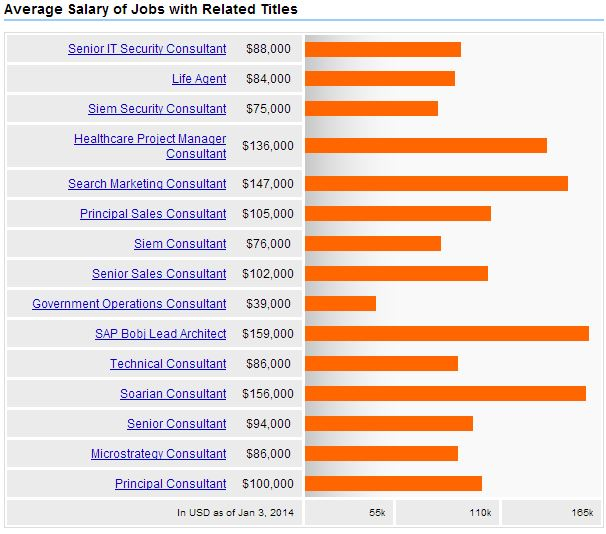
\includegraphics[width=0.7\linewidth]{./images/Techn_Cons_Sal}
				\caption{Jahresgehalt von IT-Consultants in USA}
				\label{fig:TechConsSal}
				\end{figure}\\
				%Wo ist Quelle???
		``Ein europäisches Gehalt in EUR ist ungefähr 1:1 vergleichbar mit einem 
		amerikanischen Gehalt in USD. Es wäre nicht richtig, den offiziellen Umrechnungskurs anzusetzen, da die Lebenshaltungskosten in USD in den USA mit den Lebenshaltungskosten in EUR in Europa vergleichbar sind`` \cite{InfoUSArbVertr}. In der IT-Branche wird oft ein Provision angeboten, die von erfolgreichen 
		Projekten abhängt. Das Gehalt wird in zwei Raten ausbezahlt, in der Regel am 15. und am letzten Tag des Monats.\\ \\
	\textbf{Hierarchie} \\ \\
	Gemäß US-Internetportal ``hierarchystructure.com`` \cite{HierarchieUSA} gehört die US- Geschäftshierarchie zu den erfolgreichsten Geschäftshierarchien der Welt und wird von vielen Ländern als Vorbild genommen, um das wirtschaftliche Wachstum zu erzielen. Geschäftsstruktur und Hierarchie einer Organisation werden mit dem Zweck das Gruppenziel zu erreichen aufgebaut, wobei jeder einzelne Mitglied der Organisation unterstützt wird. Dabei werden die Positionen, Aufgaben und zugehörigen Mitarbeiterrollen klar definiert.
\begin{figure}[ht]
\centering
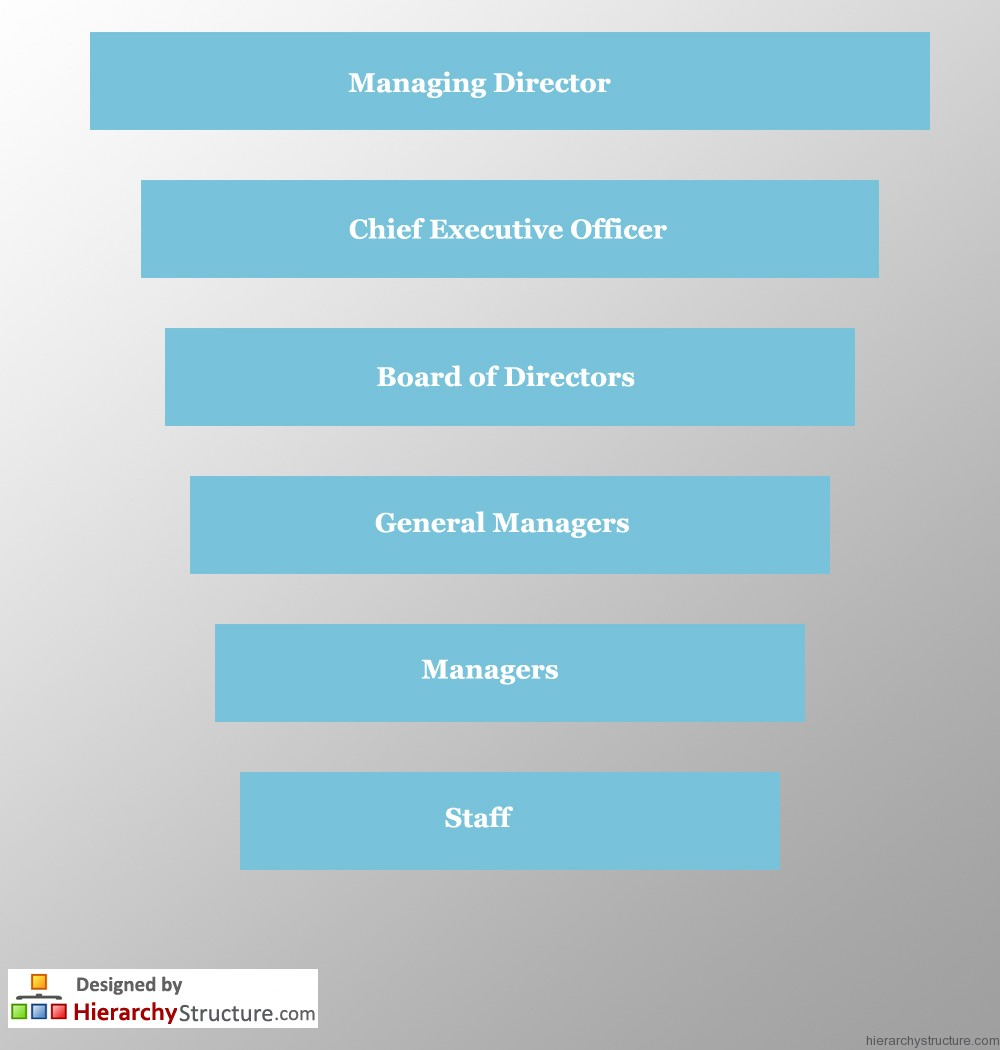
\includegraphics[width=0.7\linewidth]{./images/USA-Business-Hierarchy}
\caption{Geschäftshierarchie USA \cite{HierarchieUSA}}
\label{fig:USA-Business-Hierarchy}
\end{figure}


	\subsubsection{Deutschland}
	In allen beschriebenen Ländern unterscheidet sich erheblich der Formalisierungsgrad der Arbeitskultur. In Deutschland wird das Verhaltensweisen und Standards der Arbeitskultur sehr formalisiert in Form von gesetzlichen Vorschriften definiert. In Japan weist die Arbeitskultur auch einen hohen Formalisierungsgrad auf. Das hat nicht mit gesetzlichen Regelungen wie in Deutschland, sondern eher mit traditionellen Verhaltensweisen zu tun \cite[236]{3LaenderVergl}. Es gibt noch 2 weiteren Eigenschaften, die die deutsche Arbeitskultur bezeichnen. Dazu zählen die direkte Kommunikationsart und gründliche Planung.\\ \\
	\textbf{Pünktlichkeit}\\ \\
	Pünktlichkeit sowie gründliche Planung gehören zu den Stärken der Deutschen. IT-Consultants sind oft keine Ausnahme. Die Termine sollen gründlich geplant werden, bevor man zur Verhandlung kommt. Natürlich müssen die Termine zeitlich eingehaltenen werden. Es wird bei der Planung meist eine Pufferzeit eingerechnet, falls es trotz der aufwändigen Planung zu den zeitlichen Verzögerungen kommen soll.\\ \\
	\textbf{Arbeitszeit, Urlaub, Work-Life-Balance 
	} \\ \\
	Auch die  Trennung zwischen dem privaten und beruflichen Leben zeichnet die  deutsche Arbeitskultur aus. Im Gegensatz zu China oder Russland, wo das Arbeitsteam oft als 2. Familie eingesehen ist, hat Deutschland an dieser Stelle einen formalistischen Charakter. Trotz allem was ein Team zusammen erlebt, heißen Teammitglieder unter einender ``Arbeitskollegen``. Laut ``Germany Trade and Invest``
	Gesellschaft für Außenwirtschaft und Standortmarketingsind sind die private Einladungen von Geschäftspartner in Deutschland sehr selten, sofern nicht langjährigen Geschäftsbeziehungen bestehen \cite{ArbKulturDE}. Ob diese Tatsache eine besondere Auswirkung auf Beratungsgeschäft hat, ist nicht leicht differenzierbar. An dieser Stelle besteht ein Bedarf zur Forschung. \\
	Wie schon in vorigen Kapiteln erwähnt wurde, beträgt die gesetzlich geregelte Arbeitszeit in Deutschland 40 Stunden pro Woche. Montags bis Donnerstags sind die IT-Berater oft beim Kunde vor Ort und sind zeitlich sehr ausgelastet. Das hat damit zu tun, dass die Berater, wenn sie schon beim Kunde sind, versuchen möglichst viele Probleme zu lösen. Das führt nicht selten zu den Überstunden, die am Freitag entweder durch ein Meetings-Tag im Büro oder ein Selbststudium-Tag im Home-Office kompensiert werden. Am Freitag werden beispielsweise auftretende Probleme während des Beratung analysiert und neue Lösungen vorgeschlagen. Die Work-Life-Balance, was bei vielen Unternehmen heutzutage das Modethema ist, entspricht meisten nicht den Erwartungen von den Junior-Beratern \cite{JNRBer}. 
	Manche IT-Beratungsfirmen, meistens sind es die größten Firmen, verteilen die Projekte nach einem Senioritätsprinzip. Das bedeutet, dass ältere Berater oder die Berater, die länger im Unternehmen sind und eine Familie besitzen, öfter in den lokalen Projekten tätig sind. Damit wird oft erreicht, dass solche Berater mehr Zeit für Freunde oder Familie haben, indem sie nicht so oft reisen wie die anderen und sogar eine Möglichkeit haben in der Woche zu Hause übernachten.\\
	Arbeitstage beginnen in Deutschland im Vergleich zu den anderen Ländern wie Russland, wo meisten Büros nur ab 10 Uhr geöffnet sind, sehr früh. Bürozeiten ab 7 Uhr sind keine Seltenheit \cite{ArbKulturDE}. %Dieser Rhythmus wurde für meisten IT-Berater sehr gut eignen, weil man wegen der Einbindung an vielen Personen, alle    
	
	\textbf{Gehalt} \\ \\
	Die Gehälter von deutschen IT-Berater werden von vielen Faktoren beeinflusst. Dazu zählen die Größe, Branche und Region des Unternehmens sowie das Abschluss und das Tätigkeitsfeld, individuelle Fähigkeiten des IT-Consultants und andere Faktoren. Allgemein werden die IT-Berater sehr gut bezahlt. IT-Projektleiter, IT-Sicherheitsexperte, sowie IT-Berater verdienen am besten im deutschen IT-Umfeld \cite{VerdienstITinDE}.\\
	Senior IT-Berater aus Deutschland verdient durchschnittlich 6.250 € monatlich. Der deutsche Junior-Berater ohne Erfahrung in Beratungsbranche verdient ca. 3750 € im Monat .\cite{GehaltSAPBerDE} \\
	Die deutschen Berater, die nach Ausland geschickt werden, haben eine separate Vergütung über das gesetzliche Tagesgeld.
	\newpage
	\textbf{Lebensstandard} \\ \\
	Laut der Ranglsite für den Lebensstandard und Pro-Kopf-Einkommen von Jones und Klenow, die im Jahr 2010 für 134 Staaten ausgerechnet wurde, steht Deutschland auf dem 2.Platz nach USA (sieh Kapitel Japan - Gesetze: Steuer und Lebensstandard \label{LebStdProKEink}). Trotz dieser Rangliste sinkt der Lebensstandard in Deutschland seit Euro-Einführung immer noch. Im Vergleich zu den europäischen Südländern wie Portugal oder Spanien, haben die Kernstaate der EU wie Deutschland deutliche Verluste nicht nur am Einkommen \cite{SteigungDELebstd}.\\
	Interessant zu wissen sind die Faktoren, die für deutsche Bevölkerung den Lebensstandard maßgeblich beeinflussen. Gemäß dem Online-Statistikportal statista, sind folgende Dinge (sieh Abb. 4.7) zu leisten, damit man einen akzeptablen Mindestlebensstandard in Deutschland hat.

\begin{figure} [hp]
\centering
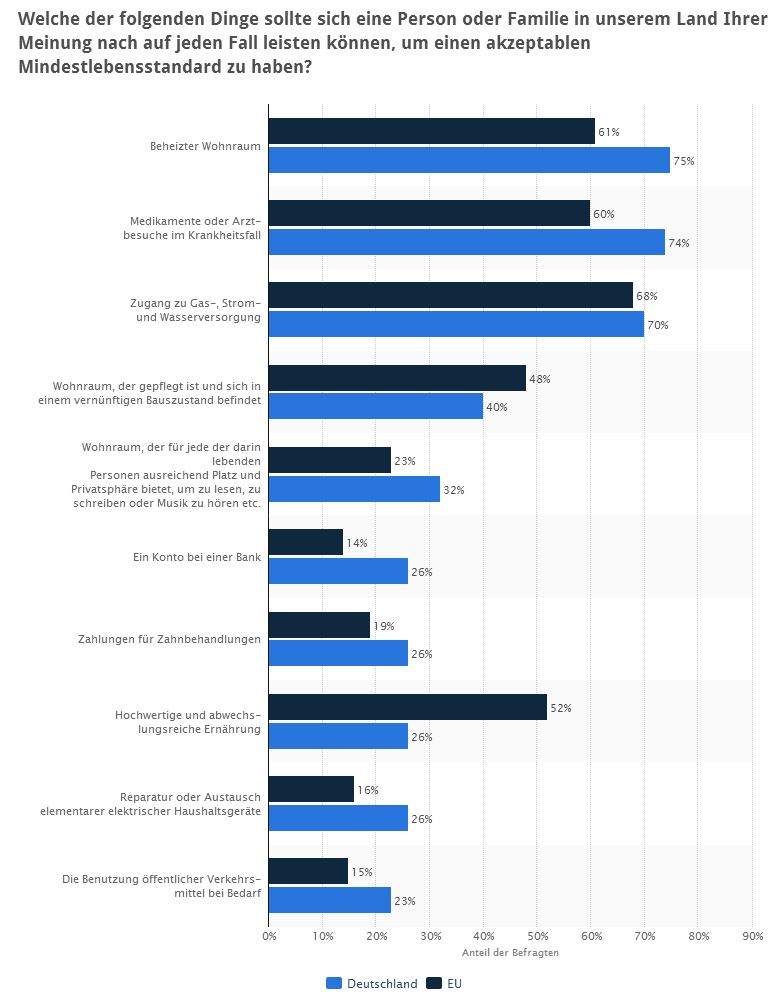
\includegraphics[width=0.7\linewidth]{./images/FaktorenLebensstand}
\caption{Faktoren des Lebensstandards in Deutschland \cite{statistaDeLebnst}}
\label{fig:FaktorenLebensstand}
\end{figure}
%\textbf{Hierarchie}
\subsection{Abschluss und Vergleich}
Zum Schluss werden wir die Arbeitskultur-Matrix überarbeiten, um festzustellen, welche Teilaspekte informationsreich sind und welche den Forschungsbedarf haben. Danach vergleichen wir einige Teilaspekte und interessanten Fakten von den ausgewählten Ländern, um Rückschlüsse auf IT-Beratungsgeschäft zu bilden.
\begin{table}[htp]
\begin{tabular}{|c|c|c|c|c|c|}
\hline  Aspekt/Land& Deutschland & USA & Russland & Japan & Indien \\ 
\hline 	Hierarchien  & z & ja & ja & ja &  z \\ 
\hline  Gehalt& ja & ja & ja & ja & z \\ 
\hline  Gesetze& z & ja & ja & ja & z  \\ 
%\hline  Grad des intuitiven Handelns& ? & ? & ? & ? & ? & ? \\ 
\hline  Kritikfähigkeit& z & z & z & ja & z \\ 
\hline  Team& ja & ja & ja & ja & z\\ 
\hline  Entscheidungsfindung& x & x & ja & ja & z  \\ 
\hline  Lebensstandard& ja & ja & ja & ja & z \\ 
\hline  Pünktlichkeit& ja & z & ja & ja & z\\ 
\hline  Arbeitszeit, Urlaub, W-L-B& ja & ja & ja & ja & z\\ 
\hline 
\end{tabular} 
\caption{Matrix der Arbeitskultur 2}
\end{table}	\\
Um die überarbeitete Matrix richtig verstehen zu können, muss man zuerst die einzelnen Symbolen definieren. Das Symbol ``Ja`` bedeutet, dass die Information über dem Teilaspekt bezüglich der IT-Beratung im internationalem Kontext vorhanden war und man daraus einen Vergleich über den gleichen Teilaspekt in ausgewählten Ländern machen kann. Das ``x`` bedeutet, dass man entweder die Information nicht vollständig hat oder, dass es keine eindeutige Beziehung zum unseren Thema gibt. Beispielsweise gibt es genug Information zu den deutschen Gesetzten, trotzdem gibt es hier keine Besonderheit, die den Beratungsprozess in irgendwelcher Weise beeinflussen kann. Das ``z`` bedeutet, dass es aus zeitlichen Gründen keine Information gefunden wurde. Dazu gibt es mehrere Gründe wie bspw. die zeitliche Begrenzung des Projekts sowie knappe Ressourcen in Form von Projektmitgliedern. Der weitere Grund liegt daran, dass es wichtiger war bei einer Zeitmangel die Prioritäten zu setzten und die anderen Teilaspekte, die relevanter waren, weiter und detaillierter zu betrachten.\\ \\
Einer der wichtigsten Teilaspekten war das Gehalt der IT-Berater. Wenn wir die Gehälter von den Senior-Berater in den ausgewählten Ländern vergleichen, dann kann man vermutlich sagen, dass die Senior-IT-Berater aus Deutschland am meisten verdienen.
\begin{table}[htp]

\begin{tabular}{|c|c|c|c|c|}
\hline Land & Deutschland & USA & Japan &  Russland\\ 
\hline durch. Gehalt in € & 75.000 & 63.537 & 56.804 &  46.140\\ 
\hline 
\end{tabular} 
\caption{IT-Berater-Gehalt in ausgewählten Ländern}
\end{table}

Wenn wir das Gehalt in Beziehung mit dem Lebensstandard	in diesen Ländern betrachten. Dann können wir vermuten, dass die Lebenshaltungskosten in Russland billiger sind als in Deutschland. Wenn wir das Gehalt und Lebensstandard ins Verhältnis setzen, dann ergibt sich ganz andere Gehälter-Ranking: Russland->Deutschland-> USA -> Japan.
\begin{figure}[ht]
		\centering
		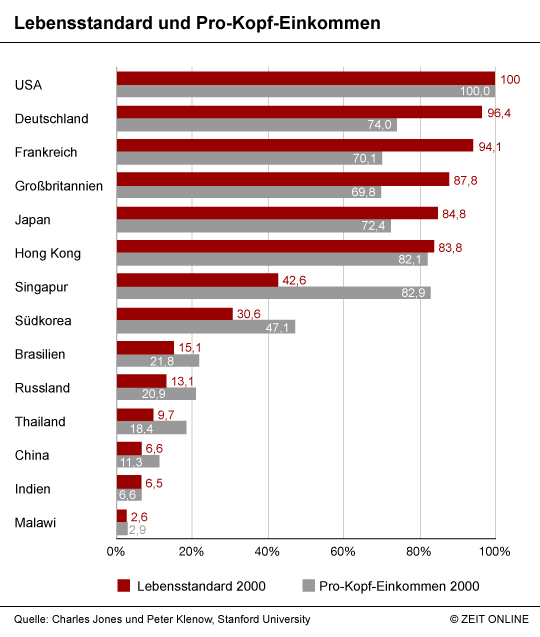
\includegraphics[width=0.7\linewidth]{./images/Lebensstandard-Pro-Kopf-Einkommen}
		\caption{Lebensstandard und Pro-Kopf-Einkommen \cite{LebensStd}}
		\label{fig:LebStdProKEink}
		\end{figure}
Wenn unsere Vermutungen richtig sind, dann arbeiten IT-Berater aus Japan mit dem Abstand am meisten. Im Allgemeinen arbeiten IT-Berater in den ausgewählten Ländern recht viel. Der Grund liegt an dem Beruf des Beraters und seinen spezifischen Eigenschaften wie Kundennähe, Reisebereitschaft usw. Um eine gute Work-Life-Balance zu erreichen, müssen Berater viel Selbstdisziplin haben, um die private Zeit ordentlich zu verwalten.\\
Wenn wir den Aspekt ``Gesetze`` betrachten, dann können wir abschließend sagen, dass es einige interessante Fakten in den ausgewählten Ländern gibt. Steuern und Sozialabgaben sind in Japan beispielsweise billiger als in Deutschland, in den USA gibt es Besonderheiten im Arbeitsgesetz (keine Kündigungszeit aufgrund der kleinen Probezeit), in Russland gibt es eine Besonderheit bei der Personalauswahl(``unser Mann``) und die Gesetze haben meistens keinen eindeutig verbindlichen Charakter.\\
Wenn wir den Aspekt Team analysieren, dann kann man nachträglich sagen, dass einige Besonderheiten bei der Gruppenarbeit im Beratungsgeschäft in diesen Ländern gibt. In Russland sowie in Japan wird der Team , in diesem Fall passt der Begriff ``Arbeitskollektiv`` am besten, von den historischen und kulturellen Eigenschaften des Volkes stark beeinflusst. Im Gegensatz zu diesen beiden Ländern gibt es in den westlichen Ländern Deutschland und USA einen modernen Team mit der Gleichberechtigung aller Teammitglieder.\\
Abschließend lässt sich sagen, dass es sehr wichtig war den Aspekt der Arbeitskultur für den internationalen Beratungsprozess zu analysieren und zu vergleichen. Denn die Arbeitskultur beeinflusst nicht nur das Geschäftsleben von IT-Berater, sondern auch deren Privatsphäre. Es hat sich auch viele Unterschiede sowie einige Gemeinsamkeiten zwischen ausgewählten Ländern bezüglich der Arbeitskultur im IT-Beratungsgeschäft herauskristallisiert. Es gab auch einige interessante Fakten, die für IT-Berater gut zu wissen sind, falls sie international agieren. Das wichtigste an dieser Stelle ist noch mal zu sagen, dass man die fremde Arbeitskultur als IT-Berater im internationalen Umfeld nicht unterschätzen soll.






%neu Matrix-die ausgefüllt wird, mit umformulierten Teilaspekten. Begrüdnung:
%Durch einer Recherchewerden einige Teilaspekte verändert. Dafür gibt es mehrere Gründe, bspw. waren die recherchierten Teilaspekte besser formuliert oder einige waren in ihrer Definition zu weit gefasst und müssten demzufolge zusammengefasst werden. Für bestimmte Teilaspekte gibt es keine Information, die durch Recherche in 3 verschiedenen Sprachen (Deutsch, Englisch und Russisch) nicht zu finden ist. An dieser Stelle besteht noch Forschungsbedarf. \\
%1)Hierarchien->Hierarchien(plus Organisation) 2)Kundenverh weg 3)spezielle Rechtslage->Gesetze 4)Grad des intuitiven Handelns weg 5) Kritikfähigkeit nur bei Japan,De 6) Lebensumstände ->Lebensstandards ->Zeitmanagement in Form von Pünktlichkeit 7)Work-Life-Balance-> Arbzeit und Urlaub(Work-Life-Balance wird ersichtlich) 8)tagesrythmus gehört zur Arbeitszeit und Urlaub
